\subsection{Идея}

Чтобы распределить переменные по $N$ регистрам, в статье Чайтина предлагается:

\begin{enumerate}
    \item Построить граф зацепленности. \label{chatin_algo_build_graph}
    \item Последовательно удалить все вершины графа, помещая их в стек (уменьшая тем самым степени других вершин) в соответствии с приведенными правилами: \label{chatin_algo_choice}
    \begin{enumerate}
        \item Если существует вершина со степенью, меньшей $N$, убираем её из графа и помещаем в стек, затем переходим к пункту \ref{chatin_algo_choice}.
        \item Если граф стал пустым, переходим к пункту \ref{chatin_algo_color_assignment}.
        \item В противном случае выбираем вершину со степенью, превышающей $N$, и убираем её (выполняем выгрузку соответствующей переменной). 
        При этом необходимо обеспечить механизм выгрузки вершины из памяти перед её использованием и последующей загрузки обратно. 
        После этого переходим к пункту \ref{chatin_algo_build_graph}. \label{chatin_algo_spill}
    \end{enumerate}
    \item Извлекать вершины из стека по одной, возвращать их в граф и присваивать каждой цвет. \label{chatin_algo_color_assignment}
\end{enumerate}

Рассмотрим детали процесса.
Сначала необходимо простроить граф зацепленности.
Далее убираем все вершины, у которых число соседей меньше $N$. 
Важно отметить, что это действие не влияет на \textit{хроматическое} число графа. 
Действительно, если у вершины меньше $N$ соседей, всегда существует цвет, который можно ей присвоить. 
Это упрощает задачу, так как такие вершины можно удалить. 
После этого остаются только вершины с числом соседей не менее $N$.

Теперь необходимо выбрать одну из вершин для удаления.
Принцип выбора, предложенный Чайтиным, заключается в следующем: для каждой вершины вычисляется значение, называемое стоимостью выгрузки. 
Сначала определяем количество объявлений и использований вершины, учитывая вес каждого объявления и использования. 
Предполагается, что вес использования или объявления переменной в цикле равен 10. 
Затем, для вычисления стоимости выгрузки вершины, вычисляем отношение 
\textit{количества использований} к \textit{степени вершины}.

При выборе вершины для выгрузки выбираем вершину с наименьшей стоимостью выгрузки.

Затем необходимо перестроить граф зацепленности,
поскольку после добавления кода для выгрузки граф изменится.
После этого нужно ещё раз попытаться раскрасить граф.

Рассмотрим, как раскрасить граф, если известно, что его можно раскрасить в $N$ цветов.
Для этого каждый раз, когда вершина удаляется из графа, будем помещать её в стек.
Когда граф станет пустым, начнём извлекать вершины из стека по одной и выбирать для каждой цвет так,
чтобы никакая соседняя вершина не имела того же цвета.

Это всегда возможно, так как на момент помещения вершины в стек её степень была меньше $N$, что гарантирует наличие свободного
цвета. Таким образом, мы получим корректную раскраску графа, а вместе с ней — распределение регистров.

\subsection{Проблемы в алгоритме Чайтина}

В этом алгоритме есть проблемы, которые обнаружил и исправил Бриггс в своей работе~\cite{briggs1994}.
Рассмотрим несколько примеров.

Проанализируем граф, представленный на рисунке~\ref{fig:ex2}. Очевидно, что данный граф допускает раскраску в два цвета.  
Тем не менее алгоритм Чайтина не способен обнаружить такую раскраску и выгрузит одну из вершин.

\begin{figure}[H]
    \centering
    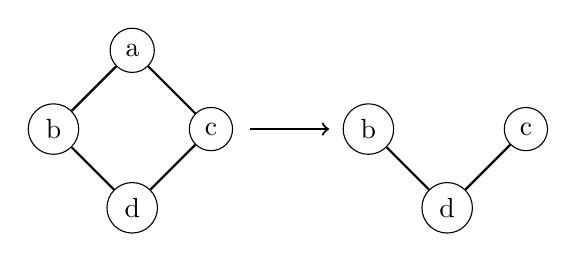
\begin{tikzpicture}
        \node[circle, draw] (a) at (2, 1) {a};
        \node[circle, draw] (b) at (1, 0) {b};
        \node[circle, draw] (c) at (3, 0) {c};
        \node[circle, draw] (d) at (2, -1) {d};
        
        \draw[thick] (a) -- (b);
        \draw[thick] (a) -- (c);
        \draw[thick] (b) -- (d);
        \draw[thick] (c) -- (d);

        \draw[->, thick] (3.5, 0) -- (4.5, 0);

        \node[circle, draw] (b1) at (5, 0) {b};
        \node[circle, draw] (c1) at (7, 0) {c};
        \node[circle, draw] (d1) at (6, -1) {d};

        \draw[thick] (b1) -- (d1);
        \draw[thick] (c1) -- (d1);
    \end{tikzpicture}
\end{figure} % Нужна ли эта картинка

Еще один пример неэффективной работы алгоритма Чайтина — это алгоритм SVD-разложения.  
В данном алгоритме используются несколько долгоживущих переменных,
то есть интервалы жизни этих переменных включают почти весь CFG программы.
Также программа содержит вложенные циклы.
Проблема распределения регистров возникает из-за долгоживущих переменных.  
Однако, поскольку стоимость выгрузки долгоживущих переменных высока, первыми выгружаются переменные циклов.  
Это не решает проблему, так как она не связана с переменными циклов.  
В результате некоторые регистры могут оставаться свободными, несмотря на выгрузку переменных циклов в память,  
что дополнительно снижает эффективность работы программы.

На рисунке~\ref{fig:structure} представлена приблизительная структура кода.

\begin{figure}[h]
    \centering
    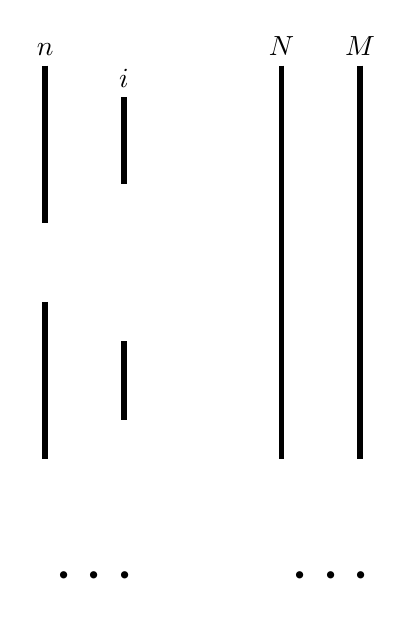
\begin{tikzpicture}
        \node[above] (n) at (0, 6) {$n$};
        \draw[line width=2pt] (n) -- (0, 4);

        \node[above] (i) at (1, 5.6) {$i$};
        \draw[line width=2pt] (i) -- (1, 4.5);

        \node[above] (N) at (3, 6) {$N$};
        \draw[line width=2pt] (N) -- (3, 1);

        \node[above] (N) at (4, 6) {$M$};
        \draw[line width=2pt] (N) -- (4, 1);

        \draw[line width=2pt] (0, 3) -- (0, 1);
        \draw[line width=2pt] (1, 2.5) -- (1, 1.5);
    
        \node at (0.625, -0.5) {\Huge $\cdots$};
        \node at (3.625,-0.5) {\Huge $\cdots$};

    \end{tikzpicture}
    \caption{Структура кода}
    \label{fig:structure}
\end{figure}

В данном коде переменные $i$ и $n$ являются переменными циклов.  
Также присутствуют долгоживущие переменные $N$ и $M$.  
Для упрощения можно считать, что они задают границы циклов, не участвуя непосредственно в самих циклах.

\begin{figure}[H]
    \centering
    \begin{tikzpicture}
        \node[circle, draw, minimum size=1cm] (i) at (0, 0) {$i$};
        \node[circle, draw, minimum size=1cm] (n) at (0, 2) {$n$};
        \node[circle, draw, minimum size=1cm] (N) at (2, 0) {$N$};
        \node[circle, draw, minimum size=1cm] (M) at (2, 2) {$M$};
        \node[circle, draw, minimum size=1cm] (Others) at (6, 1) {\text{Другие переменные}};

        \node[below of=i] {$\frac{6}{3} = 2$};
        \node[above of=n] {$\frac{6}{3} = 2$};
        \node[below of=N] {$\frac{150}{30} = 5$};
        \node[above of=M] {$\frac{150}{30} = 5$};
        \node[above of=Others] {$\frac{100}{27} \approx 3.7$};

        \draw (i) -- (n);
        \draw (i) -- (N);
        \draw (i) -- (M);
        \draw (n) -- (N);
        \draw (n) -- (M);
        \draw (N) -- (M);

        \draw (N) -- (Others);
        \draw (M) -- (Others);
    \end{tikzpicture}
    \caption{Граф зацепленности и стоимости выгрузки}
\end{figure}

% Предположим, что в графе имеются дополнительные переменные в количестве 27, каждая из которых используется 100 раз.  
% Переменные $i$ и $n$ имеют по 3 соседа и используются 6 раз, тогда как глобальные переменные $N$ и $M$ имеют по 30 соседей и используются 150 раз.  
% Предполагается, что граф необходимо окрасить в 2 цвета.  
% Рассчитаем стоимость выгрузки для каждой вершины:  
% $\text{cost}(i) = \text{cost}(n) = \frac{6}{3} = 2$,  
% $\text{cost}(N) = \text{cost}(M) = \frac{150}{30} = 5$,  
% $\text{cost}(\text{other}) = \frac{100}{27} \approx 3.7$.  
% Как следует из расчетов, первыми будут выгружены переменные $i$ или $n$, так как их стоимость выгрузки минимальна.

Предположим, что в графе имеются дополнительные переменные в количестве 27, каждая из которых используется 100 раз.  
Переменные $i$ и $n$ имеют по 3 соседа и используются 6 раз.
Переменные $N$ и $M$ имеют по 30 соседей, и пусть каждая из них используется 150 раз.
Будем считать что граф необходимо покрасить в 2 цвета.
Рассчитаем стоимость выгрузки для каждой вершины:
$\text{cost}(i) = \text{cost}(n) = \frac{6}{3} = 2$,
$\text{cost}(N) = \text{cost}(M) = \frac{150}{30} = 5$,
$\text{cost}(\text{other}) = \frac{100}{27} \approx 3.7$.
Как следует из расчетов, первыми будут выгружены переменные $i$ или $n$, так как их стоимость выгрузки минимальна.

\begin{figure}[H]
    \centering
    \begin{tikzpicture}
        \node[circle, draw, minimum size=1cm] (n) at (0, 2) {$n$};
        \node[circle, draw, minimum size=1cm] (N) at (2, 0) {$N$};
        \node[circle, draw, minimum size=1cm] (M) at (2, 2) {$M$};
        \node[circle, draw, minimum size=1cm] (Others) at (6, 1) {\text{Другие переменные}};
        
        \node[above of=n] {$\frac{6}{2} = 3$};
        \node[below of=N] {$\frac{150}{29} = 5.17$};
        \node[above of=M] {$\frac{150}{29} = 5.17$};
        \node[above of=Others] {$\frac{100}{27} \approx 3.7$};

        \draw (n) -- (N);
        \draw (n) -- (M);
        \draw (N) -- (M);

        \draw (N) -- (Others);
        \draw (M) -- (Others);
    \end{tikzpicture}
    \caption{Пересчитанные стоимости}
    \label{fig:chatin_problem_2}
\end{figure}

Предположим, что переменная $i$ была выгружена.
После этого в графе всё ещё остаются переменные, имеющие более двух соседей,
поэтому согласно пункту \ref{chatin_algo_spill} алгоритма необходимо выбрать следующую переменную для выгрузки.
Пересчитаем стоимости выгрузки (см. Рисунок~\ref{fig:chatin_problem_2}).
Алгоритм предлагает выгрузить переменную $n$, переменную цикла, однако это не решит проблему.
В итоге переменные $M$ и $N$ будут выгружены, как и переменные $i$ и $n$.
А так как переменные $i$ и $n$ используются в цикле, то их придется очень часто выгружать и загружать, что
значительно повлияет на производительность.
